\chapter{Problem description}
\section{Radio Astronomy topics related to observations scheduling problem}

``The largest single telescopes are antennas having diameters $d\approx 100\,[m]$. The angular resolution of diffraction-limited telescope is $\theta \approx \frac{\lambda}{d}$, where $\lambda$ is the wavelength of the received electromagnetic wave. Therefore, much bigger diameters are required to archive sub-arcsecond resolutions in radio waves. Mechanically these huge dishes are complicated to move with precision to point and track the sky sources to observe''~\cite{condon10}.

Interferometers comprising $N > 2$ smaller dishes have mitigated many practical problems found in huge single-dishes, increasing the collecting area into the order of $[km]$. Nevertheless, the interferometer requires extra electronic and computing power to correlate all the raw data coming from the antennas in real-time~\cite{condon10}.
The most basic interferometer is a pair of radio telescopes whose voltage outputs are multiplied and averaged or \textit{correlated}, which has the effect of filtering out high frequencies~\cite{thompson01}. Even the most elaborated interferometers with $N\gg2$ elements are treated as $\frac{N(N-1)}{2}$ independent interferometer pairs, each one of these pairs are called \textit{baselines}. The two antennas basic interferometer is presented in figure~\ref{fig:interferometer}. The wavefront from the source in direction $\theta$ reaches the right-hand antenna at a time $\tau_g = \frac{b}{c}\sin\theta$ before it reaches the left-hand antenna. $\tau_g$ is the geometric delay and $c$ is the speed of light.

\begin{figure}[htbp]
\centering
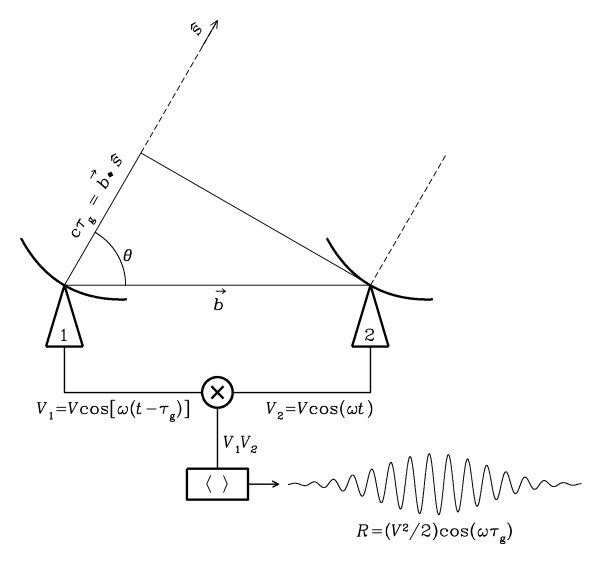
\includegraphics[width=0.5\textwidth]{images/intblock}
\caption[Two-element interferometer observing a narrow frequency $\nu=\frac{\omega}{2\pi}$]{Two-element interferometer observing a narrow frequency $\nu=\frac{\omega}{2\pi}$. Source \url{http://www.cv.nrao.edu/course/astr534/images/intblock.svg}}
\label{fig:interferometer}
\end{figure}

Then, the output voltage of antennas 1 and 2 can be written as:
\begin{eqnarray}
V_1 &=& V\cos(\omega (t-\tau_g)) \\
V_2 &=& V\cos(\omega t)
\end{eqnarray}

Then, the correlator first multiplies these two voltages to yield the product
\begin{equation}
V_1V_2 = \frac{V^2}{2}\Bigg(\cos(2\omega t - \omega \tau_g) + cos(\omega \tau_g)\Bigg)
\end{equation}
 
and finally taking a time average long enough $\Delta t \gg \frac{1}{2\omega} = T$
\begin{equation}
R = \langle V_1V_2\rangle = \frac{V^2}{2} \frac{1}{T}\int_{-\frac{T}{2}}^{\frac{T}{2}} \big(\cos(2\omega t - \omega \tau_g) + cos(\omega \tau_g)\big) dt
\propto \cos(\omega \tau_g)
\end{equation} 
 
The correlator output voltage $R$ varies sinusoidally with the change of source direction in the interferometer frame. These variations are called \textit{fringes}. Thus, in terms of frequency $\nu$, the output multiplier is proportional to
\begin{equation}
F = \cos(2\pi \nu \tau_g) = \cos\Bigg(\frac{2\pi\, b \sin \theta}{\lambda}\Bigg)
\end{equation}

A development of the simple analysis can be make if we consider two Fourier components of the received signal at frequencies $\nu_1$ and $\nu_2$. These frequencies components are statically independent so that the interferometer output is the linear sum of the responses component~\cite{thompson01}. Hence the output has component $F_1$ and $F_2$ as shown by equation~\ref{eq:sinc-fringe}. Where $l = \sin \theta$.
\begin{equation}
\label{eq:sinc-fringe}
F(l) = \frac{1}{\Delta\nu}\int_{v_0-\frac{\Delta\nu}{2}}^{v_0+\frac{\Delta\nu}{2}}\cos\Bigg(\frac{2\pi b l \nu}{c}\Bigg)dv=
\cos\Bigg(\frac{2\pi b l \nu_0}{c}\Bigg)\frac{\sin(\frac{\pi b l \Delta \nu}{c})}{\frac{\pi b l \Delta \nu}{c}}
\end{equation}
 
Thus the fringe pattern has an envelope in the form of a $sinc$ function ($sinc(x) = \frac{\sin\pi x}{\pi x}$)

The response of a two-element interferometer with directive antennas is that sinusoid multiplied by the product of the voltage patterns of the individual antennas. Normally the two antennas are identical, therefore the product is the power pattern of the much wider individual antennas, and is called the \textit{primary beam}. The primary beam is usually a Gaussian much wider than fringe period. The Fourier transform of the product of two functions is the convolution of the Fourier transforms, therefore the interferometer with directive antennas responds to a finite range of angular frequencies centered on $\frac{b\sin\theta}{\lambda}$~\cite{condon10}.

Improving the instantaneous point-source response requires more Fourier components; which means more baselines. Increasing the number of baselines have an effect over the point-source response obtained by averaging the outputs of all the pairs, which rapidly approaches a Gaussian as the number of antennas increases. The figure~\ref{fig:interf-components} presents the synthesized main beam of the two, three and four-element interferometer, which is nearly Gaussian with \textit{angular resolution} $\sim \frac{\lambda}{b}$, where $b$ is the longest baseline~\cite{condon10}.  
\begin{figure}[htbp]
\centering
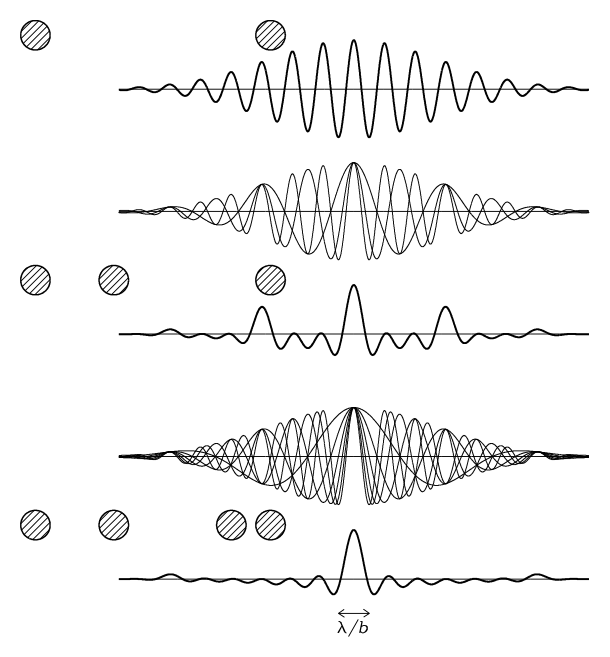
\includegraphics[width=0.5\textwidth]{images/interf4}
\caption[Instantaneous point-source responses of interferometers with overall projected length $b$]{Instantaneous point-source responses of interferometers with overall projected length $b$. Source \url{http://www.cv.nrao.edu/course/astr534/images/interf4.svg}}
\label{fig:interf-components}
\end{figure}

\subsection{Sensitivity}
\label{sec:sens}
The observation total RMS noise could be accumulated over different observation sessions, only if all the observations are done over the same target, with the same observational setup (i.e., same correlator configuration and observing frequency). The accumulated RMS noise over the time for a given setup is known as \textit{sensitivity}~\cite{avarias11}.

\subsection{Weather}

The Earth atmosphere is a layer of gases surrounding the solid mass of Earth. This layer of gases is maintained in this position due the gravitational effect of the solid mass. Most of the Earth's atmosphere is composed by Nitrogen and Oxygen used by most of the micro-organisms for respiration and some carbon dioxide used by most of the plants and other organism for photosynthesis,	also it serves as protection of ultraviolet radiation for the living organisms. Most of the mass (around $80\%$) of the atmosphere and almost all the weather phenomenon occurs in the lowest layer of the Earth's atmosphere, the \textit{Troposphere}.

The troposphere is extending from Earth's surface to 7 to 10 km of altitude, the temperature decreases with altitude in this layer, clouds form and convection can be significant. The troposphere is composed mainly of $N_2$, $O_2$, trace gases such as water vapor, $N_2O$ and $CO_2$, and particles such as liquid water and dust in clouds. Generally, the troposphere become increasingly opaque with increasing frequency as shown in figure \ref{fig:atmospheric-opacity}, mostly due the absorption by $O_2$ and $H_2O$~\cite{taylor99}.

\begin{figure}[htbp]
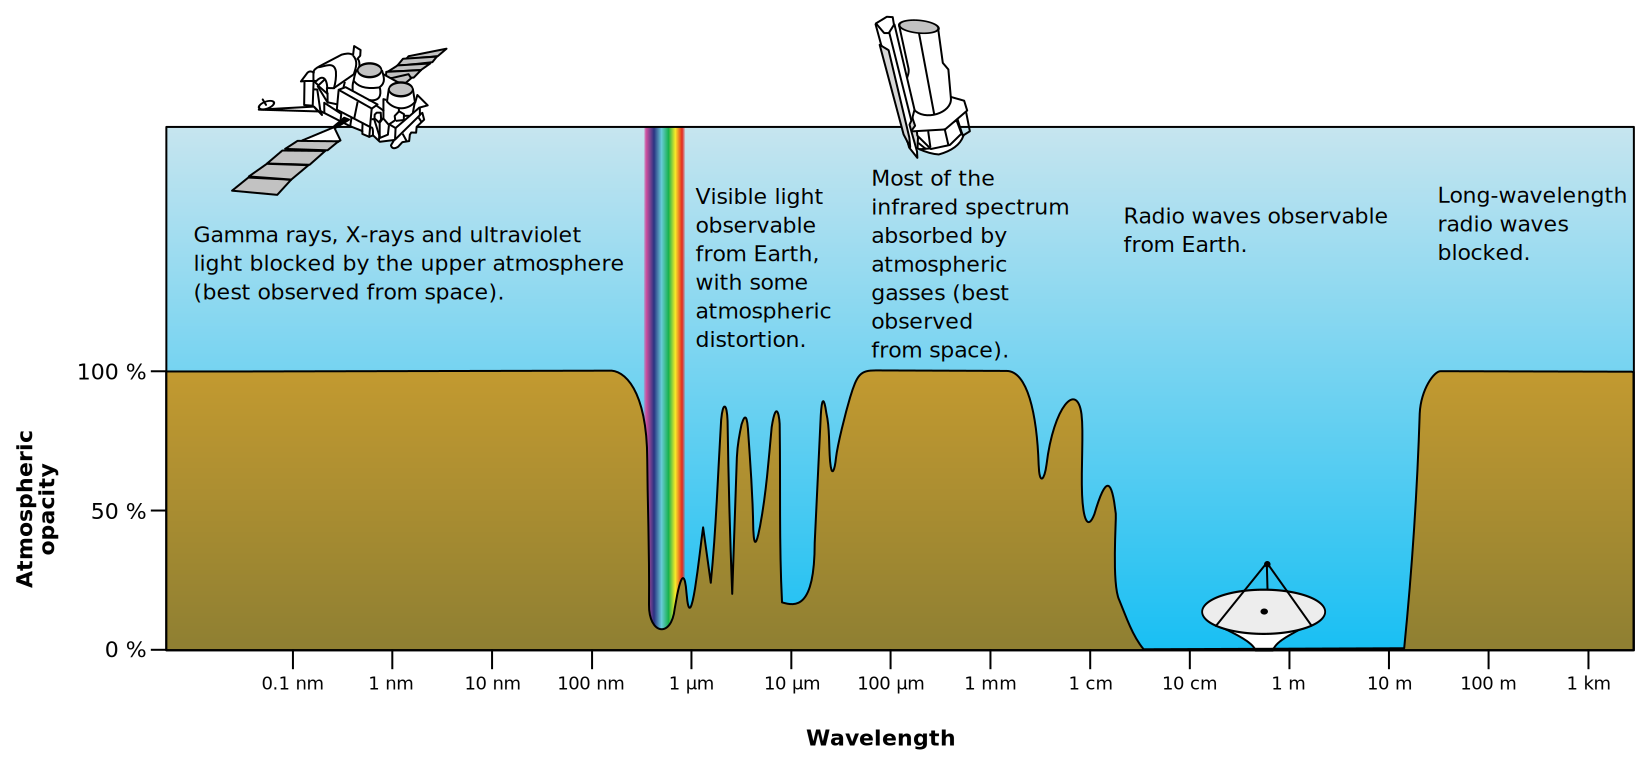
\includegraphics[width=\textwidth]{images/Atmospheric_electromagnetic_opacity}
\caption[Opacity of the Earth's atmosphere given different wavelength coming from space]{Opacity of the Earth's atmosphere given different wavelength coming from space. Source \url{http://en.wikipedia.org/wiki/File:Atmospheric_electromagnetic_opacity.svg}}
\label{fig:atmospheric-opacity}
\end{figure}

\begin{figure}[]
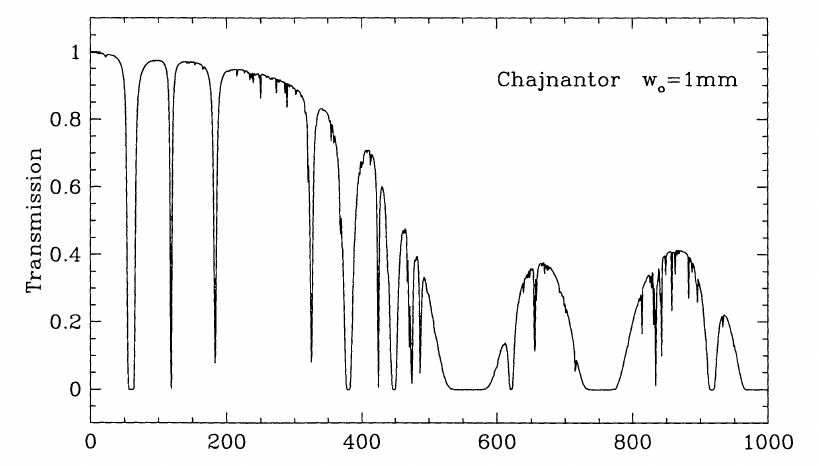
\includegraphics[width=\textwidth]{images/chajnantor-atm-transmission}
\caption[Transmission of the atmosphere from 0 to 1000 GHz for the ALMA site at Chajnantor in Chile]{Transmission of the atmosphere from 0 to 1000 GHz for the ALMA site at Chajnantor in Chile assuming the typical value of $w_0 = 1\,[mm]$ of precipitate water vapor. Source: \cite{taylor99}}
\label{fig:chaj-atm-tx}
\end{figure}

\begin{figure}[]
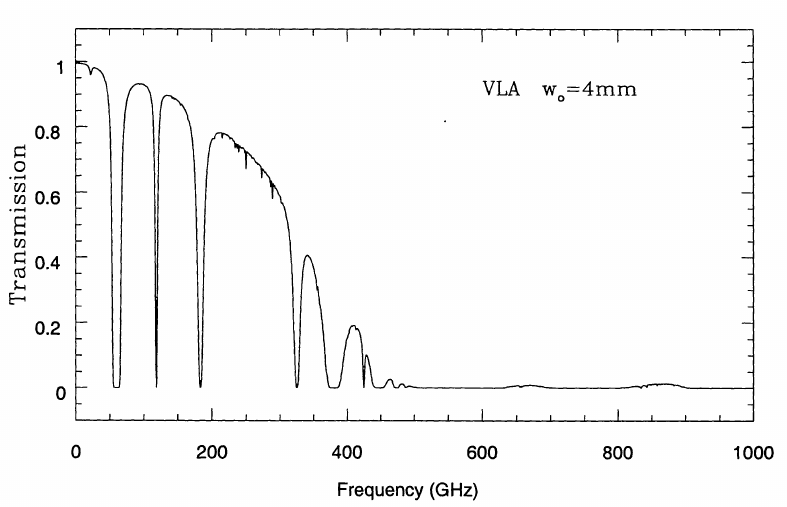
\includegraphics[width=\textwidth]{images/vla-atm-transmission}
\caption[Transmission of the atmosphere for VLA site in Socorro, NM]{Transmission of the atmosphere for VLA site in Socorro, NM, assuming a value of $w_0 = 4\,[mm]$. Source: \cite{taylor99}}
\label{fig:vla-atm-tx}
\end{figure}

Figure \ref{fig:vla-atm-tx} shows the model of the atmospheric transmission at cm and mm wavelengths for the VLA site at 2150 m of altitude, figure \ref{fig:chaj-atm-tx} shows the model for ALMA site located in Chile at 4600 m of altitude. In both plots is possible to see a strong absorption lines including the water line at 22 GHz and 183 GHz, and the $O_2$ lines at 60 GHz and 118 GHz, plus a systematic decrease in the transmission with increasing frequency between lines. Every plot includes a different value for the column density of precipitable water vapor $w_0$ where each of one is typical for the site where the samples were taken. The precipitable water vapor (PWV) is the depth of the water vapor in the atmosphere in the site if it were converted to liquid phase.

Another important parameter in radio astronomy is the \textit{System Temperature ($T_{sys}$)}, this quantity measures the overall sensitivity of the receiving system. At centimetre, millimetre wavelengths, the temperature of the receiving system dominates the system noise temperature that is the receiver and the antenna.

\section{General problem}
\newtheorem{problem-def}{Definition}
The atomic unit to be scheduled is called Scheduling Block (SB).

\begin{problem-def}
A SB is represented as a n-tuple of time independent  properties ($P$). Let $S_0$ be the set of all SBs,
$$S_0 = P_1 \times P_2 \times ... \times P_n,$$
for appropriate $P_i$ sets. Then one SB is:
$$sb = (p_1, p_2, ..., p_n) \mid p_i \in P_i$$
\end{problem-def} 

\begin{problem-def}
For a given time $t$ and a set of SBs $S \subseteq S_0$, the SB selection returns a subset of S:
$$sel:(t,S) \rightarrow \mathcal P \left({S}\right)$$
\end{problem-def}

Given these definitions, a property of $sel$ follow:

\newtheorem{sel-props}{Property}
\begin{sel-props}
The full selection operation $sel$ for a given time $t$ can be decomposed into independent selection operations, one for each property $p_i$:
$$sel(t,S) = sel_1(t, S) \cap sel_2(t, S) \cap ... \cap sel_n(t,S)$$
In general, each selection operation can be expressed as an inequality, defining the ``schedulable time window'' for a given $sb_j$:
$$sb_j \in sel_i(t, S)\,i.i.f\;\alpha_1(t, sb) \leq \alpha(t, sb) \leq \alpha_2(t, sb)$$
\end{sel-props}

Without losing generality, the inequality of the property can be separated into two inequalities, and the condition can be expressed as: 
$$\alpha'(t, sb) \leq \alpha (t, sb)$$
Regarding the dependencies of both $\alpha$ and $\alpha'$, if the property depends on $t$, then the property is \textit{dynamic}, it means that the property value to satisfy the inequality is calculated and updated accordingly the scheduling algorithm progress. On other hand the properties depending only on $sb$ are \textit{static}, therefore the values to satisfy their inequalities are pre-calculated at the beginning of the algorithm selected to solve this problem.

%\subsection{Static and dynamic constraints}

%As stated in section~\ref{sec:apdm} a target is composed by three elements, which match the constraint categories detailed here: \textit{sky source}, \textit{instrumentation} and \textit{weather}.

%In common terms a Scheduling Block is ``schedulable'' only if the representative target for the given scheduling block is observable, this means that the source of the sky is visible, the array configuration has enough hardware capabilities to observe the source according to the scientific plan, the weather conditions are good enough to carry on the observation, etc. Basically this is the intersection of the different $sel$ functions and it is defined as the \textit{schedulable time window} for a given scheduling block, this window could be available several times during the observing season. In practical terms a scheduling block can be observed as many times as possible until it has been completed.

%The description of each one of the different categories is as follow:

%\begin{description}
%    \item[Instrumentation] \hfill \\
%Every scheduling block execution is done in an \textit{Array} which is a subset of the available antennas in the observatory. Each antenna has its own hardware configuration to receive electromagnetic waves from the space. An array will have the hardware configuration common to all the antennas conforming the array, the idea is to observe the target with the same hardware in all the antennas as they were a single instrument. In general, in an observatory all the antennas conforming an array will have all the same capabilities, even they can be interchangeable between each other and should not be any difference. The array configuration and the availability of the instrumentation is decided beforehand, and for effects of the algorithm is considered a static constraint. 

%Nonetheless, problems in some instruments during observatory operations could temporally remove some capabilities from some antennas, or even the entire antenna could be removed, altering the original instrumentation properties given initially to the array. Since all these failure are not planned this is considered a dynamic constraint.

%	\item[Sky source] \hfill \\
%In general a sky source will be visible in daily basis for certain amount of time, then the source will go below horizon due the Earth's rotation, unless the source is circumpolar in which case the source will be always visible. Also the Earth's orbit movement around the sun would cause that a source will be visible during a period of the calendar year only. Both of these source properties are predictable and can be calculated before the execution of any observation.

%Every time that a observation starts, the telescope needs to be calibrated to adjust pointing corrections based on atmospheric conditions and source position. It is possible to predict how much time will be spent on calibrations, if the observation plan is given before the execution of observations starts. However sometimes, this is not the case due improvement or deterioration of the expected weather conditions,  making this constraint dependable on the time when the observation is expected to be executed.
  
%	\item[Weather] \hfill \\
%The weather cannot be foreseen with exactitude, even the most accurate weather forecast will have a error margin, which will increase if the period of time foresaw increase. Once the weather condition has changed, for good or bad, usually the list of the scheduling blocks to be observed needs to be updated accordingly. The time frame on what the algorithm can optimize the observations is bounded to the reliability of the weather pattern prediction, doing optimization beyond that could be worthless.

%\end{description}

%Another important property of every project submitted to be observed in the observing season, is that they does not have the same science value, this means there are certain projects that are more interesting to observe and complete than others. This measure of how much value has a project is given by the Time Assignment Committee at the observatory, therefore the scheduler must be aware of this and try to complete most of the projects having the ``highest'' science qualification, this will be known as the \textit{scientific value} or \textit{scientific throughput}.

\subsection{Completing Scheduling Blocks and Observation projects}
\label{subsec:completing-obs}
A scheduling block does not need to be completed in just one observation, in fact the scheduling block can be observed multiples times at different calendar time, hence different weather conditions and different array configurations as well, until the scheduling block is considered complete.
A scheduling block will be completed, and put its state as complete, if it meets any of following three criterion:
\begin{itemize}
	\item \textit{Number of repetitions}: A scheduling block can have a limit of how many times can be observed.
	\item \textit{Total time observed}: A scheduling block could have a limit of how much time can be observed.
	\item \textit{Sensitivity achieved}: As stated in section \ref{sec:sens} if the goal for the RMS noise accumulated is achieved, then the scheduling block will be considered completed.
\end{itemize} 

%The criteria to determine whether a project was completed or not, for simplicity of this study, is based in how many scheduling blocks or ObsUnit sets, belonging to the Observation project, have been completed; or the total amount of time observed, which is the sum of all the scheduling blocks observations. 
However, human intervention is required to determine whether the project has been completed, based on the quality of science data extracted from the observations. The algorithm establishing whether a observation project is completed or not for real, is far beyond the scope of this study. For this problem instance will be considered an Observation Project completed, when all its belonging Scheduling Blocks have been completed.

\subsection{Observing season (Observation cycle)}

Over the whole time available in the observing season, different \textit{Array configurations}, that can either co-exist at the very same time with other array configurations, or can be created in serial over the time frame of the observation season, or a combination of both situations.

Each array configuration can be composed of one or more antennas available at the observatory. Nonetheless, offers the capabilities common to all the antennas belonging to the array. Each array will offer basic differences i.e the angular resolution, the sensitivity achieved in every observation, which is dependent of the number of antennas in the array (see section~\ref{sec:sens}), etc. At the same time, one or more arrays can be available for observations, however each scheduling block must be observed by just one array at a given time.

\section{ALMA Scheduling}
\label{sec:alma-sched-problem}
The Atacama Large Millimeter/submillimeter Array (ALMA) is a major collaboration effort between European, North American and East Asian countries, under construction on the Chilean Chajnantor plateau, at 5.000 meters altitude. When completed, it will be the largest radio telescope on earth, with more than 60 antennas of 12 and 7 meters diameter, distributed over a wide extension, with up to 16 kilometers of baseline length. The ALMA interferometer will provide the possibility to be used as a single array, or as up to six minor independent arrays or groups of antennas. As each array is equivalent to one instrument, this can eventually be seen as a multi-telescope problem. The antennas will be changing their positions over the year, as different distributions will be used to exploit various kinds of observations. Since ALMA does not observe in the visible spectrum, observations are not limited to night time only, thus a 24/7 operation with as small downtime as possible is expected. However during commissioning operations, which is the current status of ALMA, it is expected only to use a fraction of the day and calendar year to schedule scientific operations.

ALMA will operate exclusively in service mode. Therefore, the Scheduling software Subsystem provides a fully automatic “quasi-real-time” dynamic scheduling platform, mostly with the only human participation of supervision. This Subsystem is still under development, and the algorithm(s) are still under heavy testing. The main problem is the dynamic priorities scheduling, which differs widely from the traditional dynamic job-shop problem.
The ALMA telescope will be operated as one or more antenna arrays, executing observation blocks corresponding to accepted project proposals. There will be three different antenna types, provided by three vendors:
\begin{itemize}
\item 12-m antennas (50): This is the main array to be operated, and also the one to be divided into several sub-arrays. They are provided by vendors Vertex (Vertex Antennatechnik GmbH) and AEM (Alcatel Alenia Space France, Alcatel Alenia Space Italy, European Industrial Engineering S.r.L., MT Aerospace).

\item 7-m antennas (12): This is the main part of the ALMA Compact Array (ACA), which will  operate as a separate array. They are provided by MElCo (Mitsubishi Electric Corporation).

\item 12-m total power antennas (4): These are special total power antennas able to see a full 2GHz spectrum, part of the ACA, but in principle exchangeable with any of the other 12-m antennas. They are also delivered by MElCo.
\end{itemize}

\begin{figure}	
\begin{center}
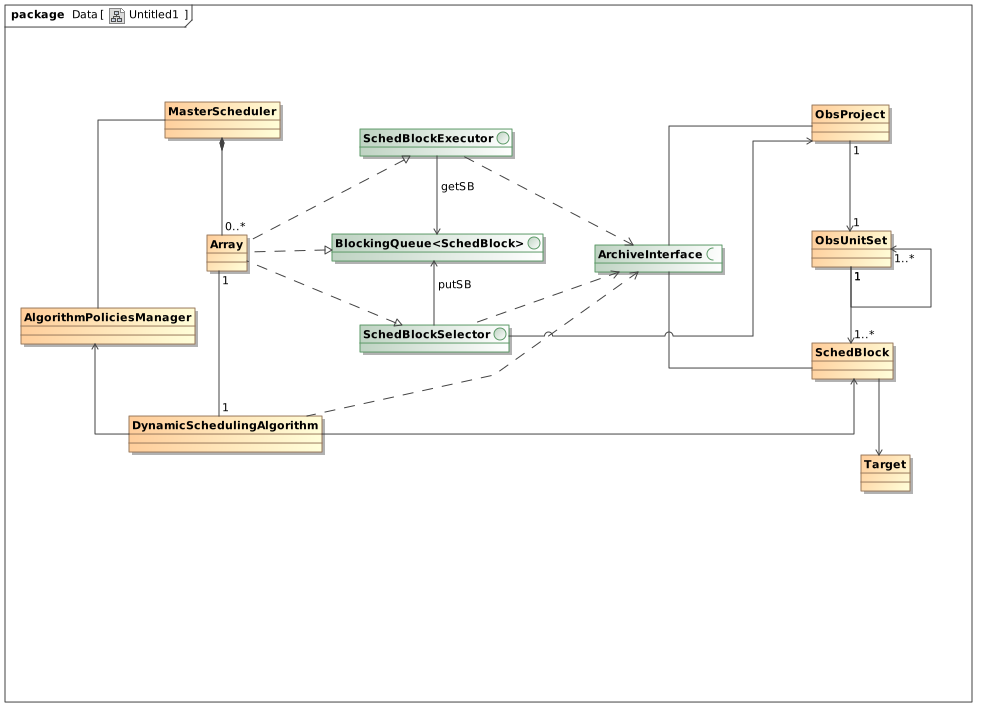
\includegraphics[width=\textwidth]{images/scheduling_class_model}
\end{center}
\caption{Basic class model of Scheduling subsystem}
\label{fig:sched-class-model}
\end{figure}

A huge part of the telescope operations will be handled through the ALMA software, which is divided into various subsystems, such as Control, Correlator (ACA and Baseline), Pipeline, Archive, Scheduling and Offline software. The big picture of ALMA Software can be seen in~\cite{schwarz04}.
The Scheduling Subsystem is the one in charge of managing antenna arrays and dynamically executing scheduling blocks. The current software design details are in~\cite{clarke12}. The basic design considers 3 main parts which are represented in figure \ref{fig:sched-class-model}: 
\begin{enumerate}
\item The ``Master Scheduler'' manages the creation of the Arrays and handle the management of the Scheduling Policies to configure the DSA.

\item  The ``Array'' is the main unit of the scheduling subsystem, each array observes Scheduling Blocks, executing them and waiting for results of the observations, finally notifying to the user of the system what has been the outcome of the observation. The Array uses directly the Archive, which is the database storing the definition of each Observation project (see appendix~\ref{sec:apdm}), through the Archive Interface. Each array has its own scheduling queue, which can contain several schedblocks waiting to be executed, but just one SchedBlock is observed at the same time in each Array.

\item The ``Dynamic Scheduler instance'' runs as a component on top of an Array, selecting the current best SB according to the algorithm policy selected for the given DSA instance.
\end{enumerate}

Each scheduling array can operate in 3 different modes:
\begin{enumerate} 
\item Manual, in this mode the scheduling queue is set with a maximum of one item, and the user is responsible to execute the observation manually using low level scripts. 
\item Automatic, in this mode the array has a unlimited size scheduling queue, once a observation has been completed a new SchedBlock is taken from this queue to observe the next one until the queue is empty or the scheduler is stopped.
\item Dynamic, in this mode the scheduling queue behaves as the array in interactive mode, but when the queue is empty, then DSA is triggered selecting the next best SchedBlock to observe, depending if the DSA is active or passive, the selected SchedBlock will be put in the queue to start the observation or the Scheduler will only notify the user, respectively. The state machine implemented as part of the current DSA can be seen in the appendix~\ref{sec:dsa-workflow} the DSA may be executed every time that a new Scheduling Block is needed to be queued, until there is no more Scheduling Blocks available.
\end{enumerate}

While most of the scheduling software will be run in the on-line software, there is a planning stage where the Scheduling algorithm plans different scenarios within a season. The on-line usage of the algorithm is known as the \textit{short-term scheduler}, this scheduler either can be used in quasi-real time or to plan observations to be carried out during a night. A \textit{medium-term scheduler} used to plan the observations for a time frame where the array configurations are the same. And finally \textit{long-term scheduler} which should be able to plan an entire season of observation across the different array configurations, ideally the algorithm should define the duration of each configuration given as a input. For the two last use cases, ALMA scientific operations uses a simulator, which is mostly described in~\cite{hoffstadt10}. Although new features have been added, the basic workflow (for more details see appendix~\ref{sec:sim-workflow}), has been kept until nowadays.

\section{Identified problems}
\label{sec:problems}
After the analysis of the different properties related to the ALMA scheduling problem it is possible to identify the following two different problems:

\begin{description}
\item[Astronomical observation scheduling] \hfill \\
Consists on determine a schedule for a given set of scheduling blocks, which all of them can be observed by the instrument, considering one array already created within a given fixed period of time. 
The idea is to generate a plan to try to observe all, or most of the projects with the highest scientific value in less amount of time possible considering all, or the most critical of the scientific requirements. It may possible to not complete all the observation projects submitted for this array configuration.

\item[Array configuration planning] \hfill \\
This problem is on top of the astronomical observation scheduling problem. It consists in try to determine a plan for the different array configurations given as input, for the given observing season and for a given set of the scheduling blocks, which can be observed in multiple array configurations. At the same time, maximizing the number of the projects with highest scientific value completed, considering all or most of the scientific requirements during the observing season, however not all the observation projects may be completed. Also it is desirable to reduce the idle time of the observatory, considering all the arrays configurations. Also is desirable to reduce the amount of idle time of the instrument.
\end{description}